El problema se puede resolver basándose en la siguiente idea:

Sea L(i) la longitud del LIS que termina en el índice i tal que arr[i] sea el último elemento del LIS. Entonces, L(i) puede escribirse recursivamente como:

$$L(i) = \begin{cases}
	1 + \max(L(j)) &  0 \le j < i \quad y \quad arr[j] < arr[i] \\ 
	
	1 & Si \quad no \quad existe \quad tal \quad j 
\end{cases}$$

Formalmente, la longitud de LIS que termina en el índice $i$ es una unidad mayor que el máximo de longitudes de todos los LIS que terminan en algún índice $j$ tal que $arr[j] < arr[i]$ donde $j < i$.

Veamos la siguiente ejemplo desarrollando el árbol de recursión considerando la siguiente colección $arr[] = \{3, 10, 2, 11\}$ la colección a la cual deseamos cacular el LIS.

% TODO: \usepackage{graphicx} required
\begin{figure}[!h]
	\centering
	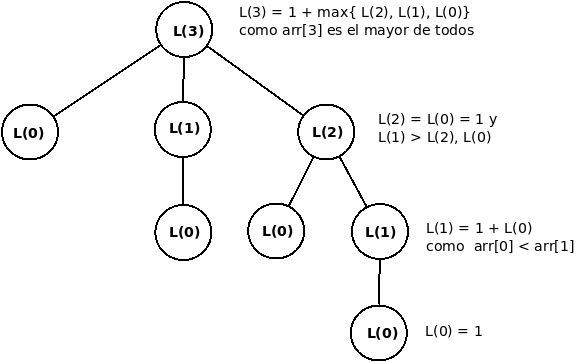
\includegraphics[width=0.7\linewidth]{img/list_recursive_tree}
	\label{fig:listrecursivetree}
\end{figure}


Veamos los pasos a seguir para implementar la idea anterior:

\begin{itemize}
	\item Crea una función recursiva.
	\item Para cada llamada recursiva, itere desde i = 0 hasta la posición actual y haga lo siguiente:
	\begin{itemize}
		\item Encuentre la longitud posible de la subsecuencia creciente más larga que termina en la posición actual si la secuencia anterior terminó en $i$.
		\item Actualice la longitud máxima posible en consecuencia.
	\end{itemize}
	\item Repita esto para todos los índices y encuentre la respuesta.
\end{itemize}

